\section{Introduction}


The widespread adoption of mobile devices has created opportunities in human-centric computing by capturing user behaviours through sensors on devices people carry. A key challenge in user modelling is the presence of shifts in human behaviours, where user behaviours can change over time. The problem of catastrophic forgetting \cite{kirkpatrick2017overcoming, aljundi2018memory, diethe2019continual, van2019three} has been a critical challenge in continual learning, in which deep learning models forget what has been learned when being trained on data with shifted distributions. Even though many approaches have been proposed to mitigate catastrophic forgetting \cite{kirkpatrick2017overcoming, li2017learning, shin2017continual, wu2019large}, most assume abundant labelled data for every new distribution, which is unrealistic for mobile sensing. Collecting quality ground truth when data is generated on the fly in wearable-based user modelling is particularly challenging.

\begin{figure}[t]
\begin{center}
   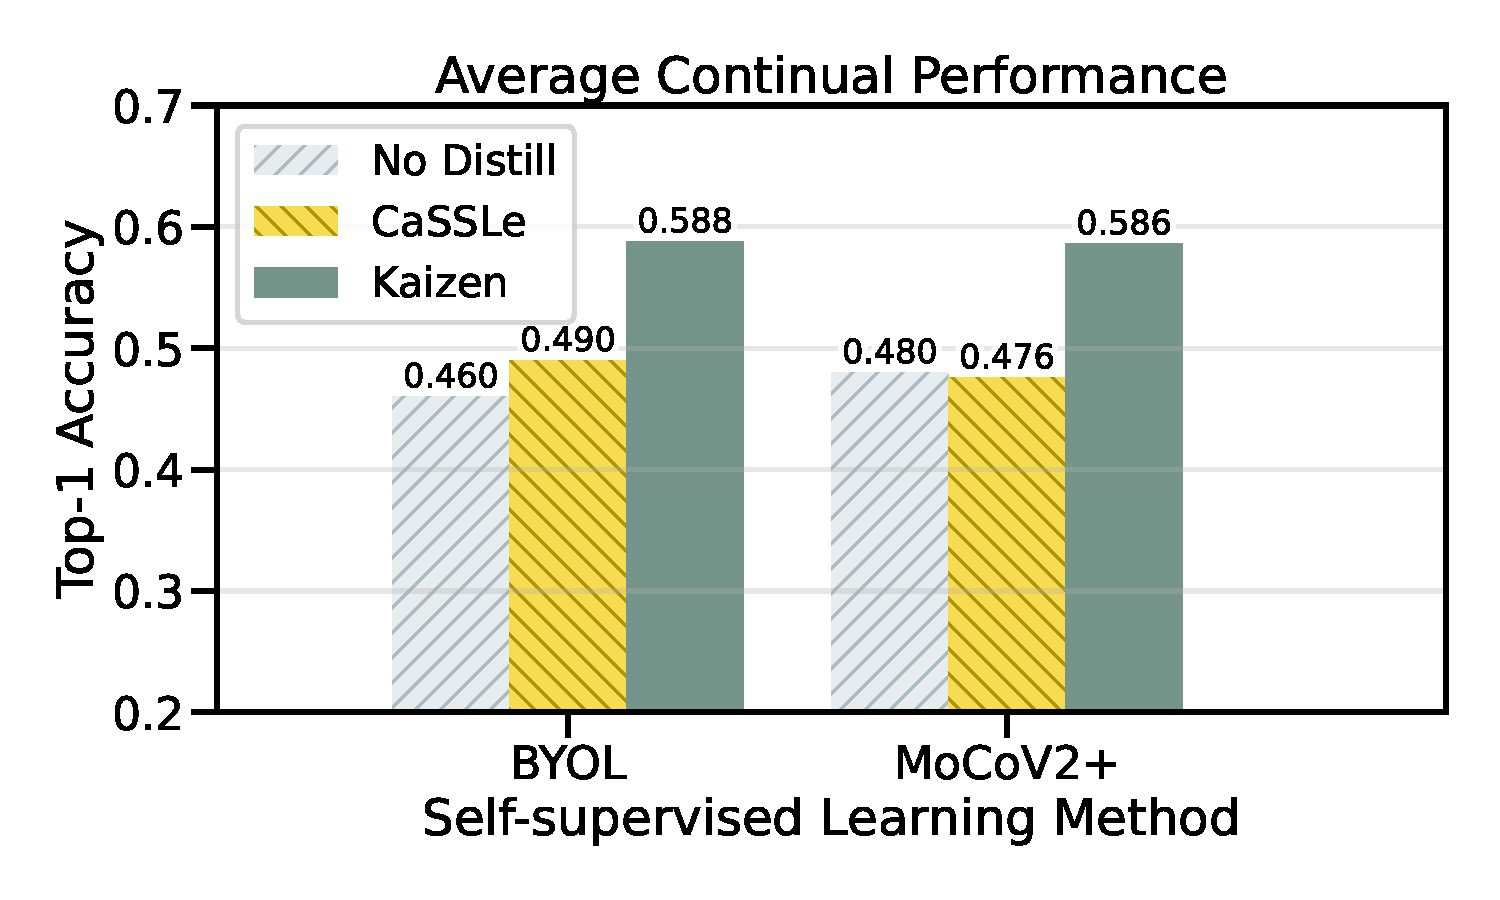
\includegraphics[width=0.7\linewidth]{figures_new/Part_1/F1-WISDM2019-6Tasks-Continual_Accuracy-v2.pdf}\\
   \vspace{-0.1in}
   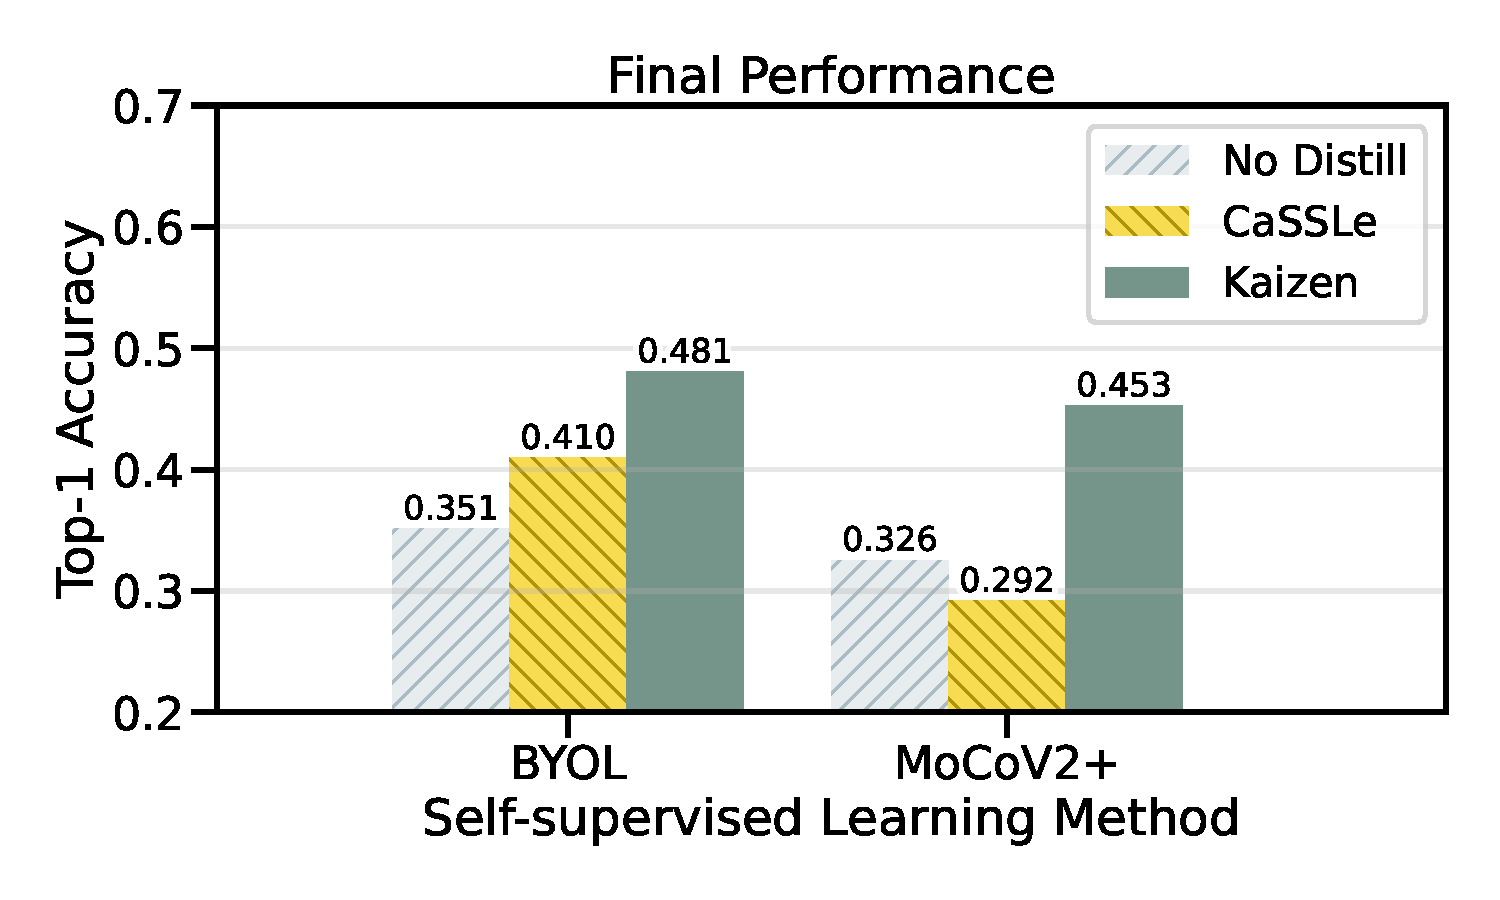
\includegraphics[width=0.7\linewidth]{figures_new/Part_1/F1-WISDM2019-6Tasks-Final_Accuracy-v2.pdf}
   
\end{center}
\vspace{-0.2in}
   \caption{Performance comparison between different training methods. Models are trained using different self-supervised learning methods and knowledge distillation strategies on class-incremental WISDM2019. The top figure shows the average performance across the entire continual learning process, while the bottom figure shows the performance in the final evaluation. 
   }
       \vspace{-0.2in}
   \label{fig:general_performance_comparison}
\end{figure}

To address this data scarcity, continual self-supervised learning (CSSL) leverages self-supervision for continual learning. Recent works \cite{fini2022self, tang2023practical} have demonstrated effectiveness in leveraging different sources of data in continual learning, proposing practical solutions with more practical data assumptions. A discussion about related work can be found in Appx.~\ref{related}.

In this study, we explore CSSL techniques for sensor-based human activity recognition. In particular, we adapted CaSSLe \cite{fini2022self} and Kaizen \cite{tang2023practical} to enable self-supervised and semi-supervised continual learning for activity recognition using accelerometer data. Beyond comparing state-of-the-art methods on comprehensive metrics, we investigated adjusting continual fine-tuning's objective importance. Balancing knowledge retention and new task learning with an adaptive weight corresponding to learned/new class ratios proved most effective for performance across tasks. This work demonstrates realistic continual learning assumptions and balancing objectives to achieve the desired performance for mobile sensing. The results highlight the trade-offs in emphasising knowledge retention or new concepts based on use cases.
